\documentclass[tikz]{standalone}
\usepackage{tikz}

\begin{document}
    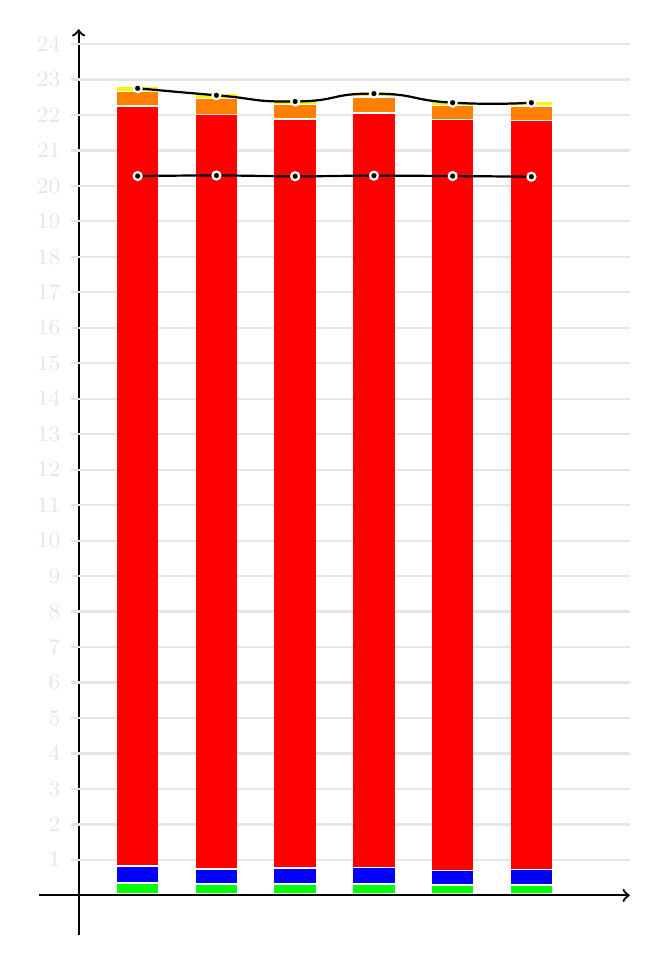
\begin{tikzpicture}[thick]
        \draw[->] (0, -0.5) -- (0, 11);
        \draw[->] (-0.5, 0) -- (7, 0);

        \draw[gray!20] (-0.1, 0.451) node[left]{\footnotesize 1}-- (7, 0.451);
        \draw[gray!20] (-0.1, 0.901) node[left]{\footnotesize 2}-- (7, 0.901);
        \draw[gray!20] (-0.1, 1.352) node[left]{\footnotesize 3}-- (7, 1.352);
        \draw[gray!20] (-0.1, 1.802) node[left]{\footnotesize 4}-- (7, 1.802);
        \draw[gray!20] (-0.1, 2.253) node[left]{\footnotesize 5}-- (7, 2.253);
        \draw[gray!20] (-0.1, 2.703) node[left]{\footnotesize 6}-- (7, 2.703);
        \draw[gray!20] (-0.1, 3.154) node[left]{\footnotesize 7}-- (7, 3.154);
        \draw[gray!20] (-0.1, 3.604) node[left]{\footnotesize 8}-- (7, 3.604);
        \draw[gray!20] (-0.1, 4.055) node[left]{\footnotesize 9}-- (7, 4.055);
        \draw[gray!20] (-0.1, 4.505) node[left]{\footnotesize 10}-- (7, 4.505);
        \draw[gray!20] (-0.1, 4.956) node[left]{\footnotesize 11}-- (7, 4.956);
        \draw[gray!20] (-0.1, 5.406) node[left]{\footnotesize 12}-- (7, 5.406);
        \draw[gray!20] (-0.1, 5.857) node[left]{\footnotesize 13}-- (7, 5.857);
        \draw[gray!20] (-0.1, 6.307) node[left]{\footnotesize 14}-- (7, 6.307);
        \draw[gray!20] (-0.1, 6.758) node[left]{\footnotesize 15}-- (7, 6.758);
        \draw[gray!20] (-0.1, 7.208) node[left]{\footnotesize 16}-- (7, 7.208);
        \draw[gray!20] (-0.1, 7.659) node[left]{\footnotesize 17}-- (7, 7.659);
        \draw[gray!20] (-0.1, 8.109) node[left]{\footnotesize 18}-- (7, 8.109);
        \draw[gray!20] (-0.1, 8.56) node[left]{\footnotesize 19}-- (7, 8.56);
        \draw[gray!20] (-0.1, 9.01) node[left]{\footnotesize 20}-- (7, 9.01);
        \draw[gray!20] (-0.1, 9.461) node[left]{\footnotesize 21}-- (7, 9.461);
        \draw[gray!20] (-0.1, 9.911) node[left]{\footnotesize 22}-- (7, 9.911);
        \draw[gray!20] (-0.1, 10.362) node[left]{\footnotesize 23}-- (7, 10.362);
        \draw[gray!20] (-0.1, 10.812) node[left]{\footnotesize 24}-- (7, 10.812);

        % MESSAGE 0
        \draw[green, fill=green] (0.5, 0.05) rectangle ++ (0.5, 0.082);
        \draw[blue, fill=blue] (0.5, 0.182) rectangle ++ (0.5, 0.168);
        \draw[red, fill=red] (0.5, 0.4) rectangle ++ (0.5, 9.596);
        \draw[orange, fill=orange] (0.5, 10.046) rectangle ++ (0.5, 0.138);
        \draw[yellow, fill=yellow] (0.5, 10.234) rectangle ++ (0.5, 0.016);
        % MESSAGE 1
        \draw[green, fill=green] (1.5, 0.05) rectangle ++ (0.5, 0.07);
        \draw[blue, fill=blue] (1.5, 0.17) rectangle ++ (0.5, 0.144);
        \draw[red, fill=red] (1.5, 0.364) rectangle ++ (0.5, 9.528);
        \draw[orange, fill=orange] (1.5, 9.942) rectangle ++ (0.5, 0.153);
        \draw[yellow, fill=yellow] (1.5, 10.145000000000001) rectangle ++ (0.5, 0.016);
        % MESSAGE 2
        \draw[green, fill=green] (2.5, 0.05) rectangle ++ (0.5, 0.068);
        \draw[blue, fill=blue] (2.5, 0.168) rectangle ++ (0.5, 0.154);
        \draw[red, fill=red] (2.5, 0.372) rectangle ++ (0.5, 9.461);
        \draw[orange, fill=orange] (2.5, 9.883) rectangle ++ (0.5, 0.137);
        \draw[yellow, fill=yellow] (2.5, 10.07) rectangle ++ (0.5, 0.012);
        % MESSAGE 3
        \draw[green, fill=green] (3.5, 0.05) rectangle ++ (0.5, 0.068);
        \draw[blue, fill=blue] (3.5, 0.168) rectangle ++ (0.5, 0.16);
        \draw[red, fill=red] (3.5, 0.378) rectangle ++ (0.5, 9.53);
        \draw[orange, fill=orange] (3.5, 9.957999999999998) rectangle ++ (0.5, 0.159);
        \draw[yellow, fill=yellow] (3.5, 10.167) rectangle ++ (0.5, 0.015);
        % MESSAGE 4
        \draw[green, fill=green] (4.5, 0.05) rectangle ++ (0.5, 0.059);
        \draw[blue, fill=blue] (4.5, 0.159) rectangle ++ (0.5, 0.131);
        \draw[red, fill=red] (4.5, 0.33999999999999997) rectangle ++ (0.5, 9.488);
        \draw[orange, fill=orange] (4.5, 9.877999999999998) rectangle ++ (0.5, 0.127);
        \draw[yellow, fill=yellow] (4.5, 10.055) rectangle ++ (0.5, 0.012);
        % MESSAGE 5
        \draw[green, fill=green] (5.5, 0.05) rectangle ++ (0.5, 0.061);
        \draw[blue, fill=blue] (5.5, 0.161) rectangle ++ (0.5, 0.142);
        \draw[red, fill=red] (5.5, 0.353) rectangle ++ (0.5, 9.463);
        \draw[orange, fill=orange] (5.5, 9.865999999999998) rectangle ++ (0.5, 0.137);
        \draw[yellow, fill=yellow] (5.5, 10.052999999999999) rectangle ++ (0.5, 0.014);

        \draw[black] plot [smooth, tension=1] coordinates { (0.75, 10.25) (1.75, 10.161) (2.75, 10.082) (3.75, 10.182) (4.75, 10.067) (5.75, 10.067)};
        \draw[white, fill=black] (0.75, 10.25) circle (0.05cm);
        \draw[white, fill=black] (1.75, 10.161) circle (0.05cm);
        \draw[white, fill=black] (2.75, 10.082) circle (0.05cm);
        \draw[white, fill=black] (3.75, 10.182) circle (0.05cm);
        \draw[white, fill=black] (4.75, 10.067) circle (0.05cm);
        \draw[white, fill=black] (5.75, 10.067)circle (0.05cm);

        \draw[black] plot [smooth, tension=1] coordinates { (0.75, 9.135) (1.75, 9.142) (2.75, 9.133) (3.75, 9.14) (4.75, 9.135) (5.75, 9.127) };
        \draw[white, fill=black] (0.75, 9.135) circle (0.05cm);
        \draw[white, fill=black] (1.75, 9.142) circle (0.05cm);
        \draw[white, fill=black] (2.75, 9.133) circle (0.05cm);
        \draw[white, fill=black] (3.75, 9.14) circle (0.05cm);
        \draw[white, fill=black] (4.75, 9.135) circle (0.05cm);
        \draw[white, fill=black] (5.75, 9.127)circle (0.05cm);
    \end{tikzpicture}
\end{document}